%%%%%%%%%%%%%%%%%%%%%%%%%%%%%%%%%%%%%%%%%%%%%%%%%%%%%%%
%
% AUTHOR:lee-shun
%
% DESCRIBTION:第三章--自动驾驶仪控制逻辑
%
%
%%%%%%%%%%%%%%%%%%%%%%%%%%%%%%%%%%%%%%%%%%%%%%%%%%%%%%%

\chapter{自动驾驶仪控制逻辑}
\label{chap:single_control_logic}
正如前文所提到的:由于文中编队控制器基于领从方法(leader-follower method),因而领机的飞行完全是由预先给定的一系列航迹点以及自动驾驶仪
所决定的。并且,本文设计的的编队控制器是以现有开源自动驾驶仪PX4的内环为基础;因此,本章将首先介绍控制领机飞行的自动驾驶导航以
及位置模块的实现逻辑,之后将介绍固定翼无人机编队飞行至关重要的基础环节-----自动驾驶仪内环,即姿态内环的实现逻辑。
内环姿态驾驶仪使用的是开源自动驾驶仪PX4。PX4是一个为无人机或者其他无人系统设计的高度模块化、可定制化的开源自动驾驶仪软件系统;
PX4软件本身提供了丰富的应用程序接口(API)以及软件开发工具包(SDK),可以与$ROS$等机器人操作系统进行数据交互。下图展示了$PX4$
的软件架构以及各个模块之间的交互关系:
\begin{figure}[H]
    \centering
    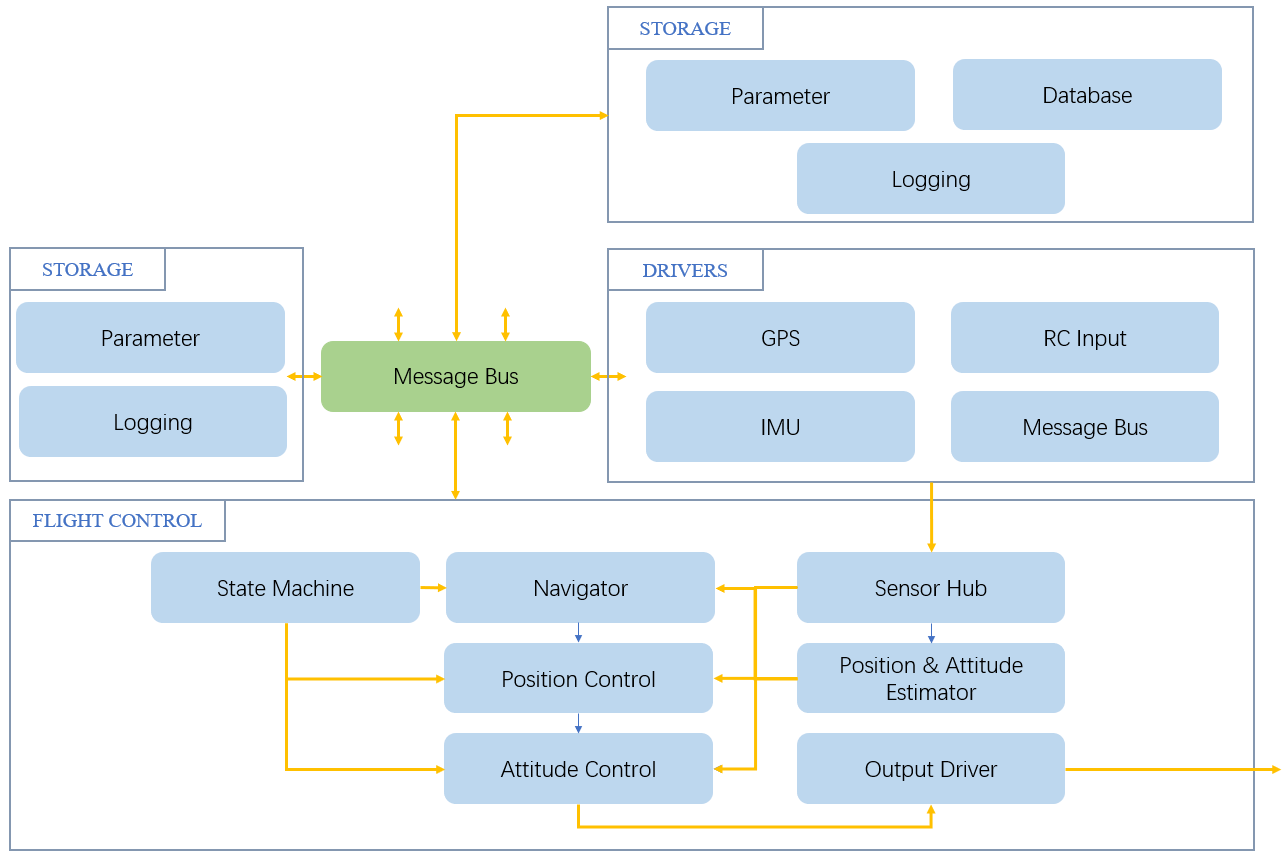
\includegraphics[width=0.8\textwidth]{figures/c4/PX4_archticher.png}
    \caption{PX4软件架构}\label{fig:PX4_archticher.png}
\end{figure}
\section{导航以及位置外环实现逻辑}
所谓导航模块(Naigator),其功能是产生相应的期望位置航点。编队中领机按照给定的航迹飞行,导航模块则根据给定的航点以及无人机的位置不断得出当前位置
下的期望航点。位置外环的主要功能是接受来自导航模块的期望位置,再结合无人机的当前位置,按照给定的导航算法,产生姿态内环的所接受的
期望姿态以及期望推力值。位置外环将无人机的运动分为竖直与水平平面的运动,并在上述两个平面内分别设计位置控制器;竖直平面控制器选用
TECS控制器,水平平面选用L1控制器。下面将简要介绍上述两种控制器的控制逻辑:
\subsection{TECS控制器控制逻辑}
所谓总能量控制(total energy control)是将无人机的速度以及高度计算得到相应的动能以及势能作为直接控制对象,应用PID控制器对动能与势能的和(total energy)
以及动能与势能的转化(total energy balance)进行控制,计算得到无人机期望俯仰角以及期望推力的控制器。飞机作为一个动力学系统,其机械能来自推力做功的输入,因而总能量控制对应着期望推力;与之对应的俯仰角控制是能量守恒的,
可作为动能向势能(反之亦然)的转化途径,对此种能量转化的控制对应着期望俯仰角。下面简要介绍$TECS$控制器的计算过程:
\\
无人机的总能量为:
\begin{equation}
    E_T=\frac{1}{2}mV_T^2+mgh
    \label{ET}
\end{equation}
对上式两边微分,可得到总能量变化率:
\begin{equation}
    \dot{E_T}=mV_T\dot{V_T}+mg\dot{h}
    \label{ET_rate}
\end{equation}
由此可得单位总能量变化率:
\begin{equation}
    \dot{E}=\frac{\dot{E}_{T}}{m g V_{T}}=\frac{\dot{V}_{T}}{g}+\frac{\dot{h}}{V_{T}}=\frac{\dot{V}_{T}}{g}+\sin \gamma
    \label{specif_ET_rate}
\end{equation}
更换式\ref{point_dynamaic}第一式形式,可得到:
\begin{equation}
    T-D=m g\left(\frac{\dot{V}_{T}}{g}+\sin \gamma\right)
    \label{point_dynamaic_change}
\end{equation}
由此可得:
\begin{equation}
    \Delta T=m g\left(\frac{\dot{V}_{T}}{g}+sin\gamma\right)
    \label{thrust}
\end{equation}
关于能量转化,定义:
\begin{equation}
    B=m g h-\frac{1}{2} m V_{T}^{2}
\end{equation}
能量转化率为:
\begin{equation}
\dot{B}=sin\gamma-\frac{\dot{V}_{T}}{g}
\end{equation}
这里参照开源软件$PX4$内部的TECS控制器设计方法,总能量环和能量分配环的控制逻辑框图如下所示:
\begin{figure}[H]
    \centering
    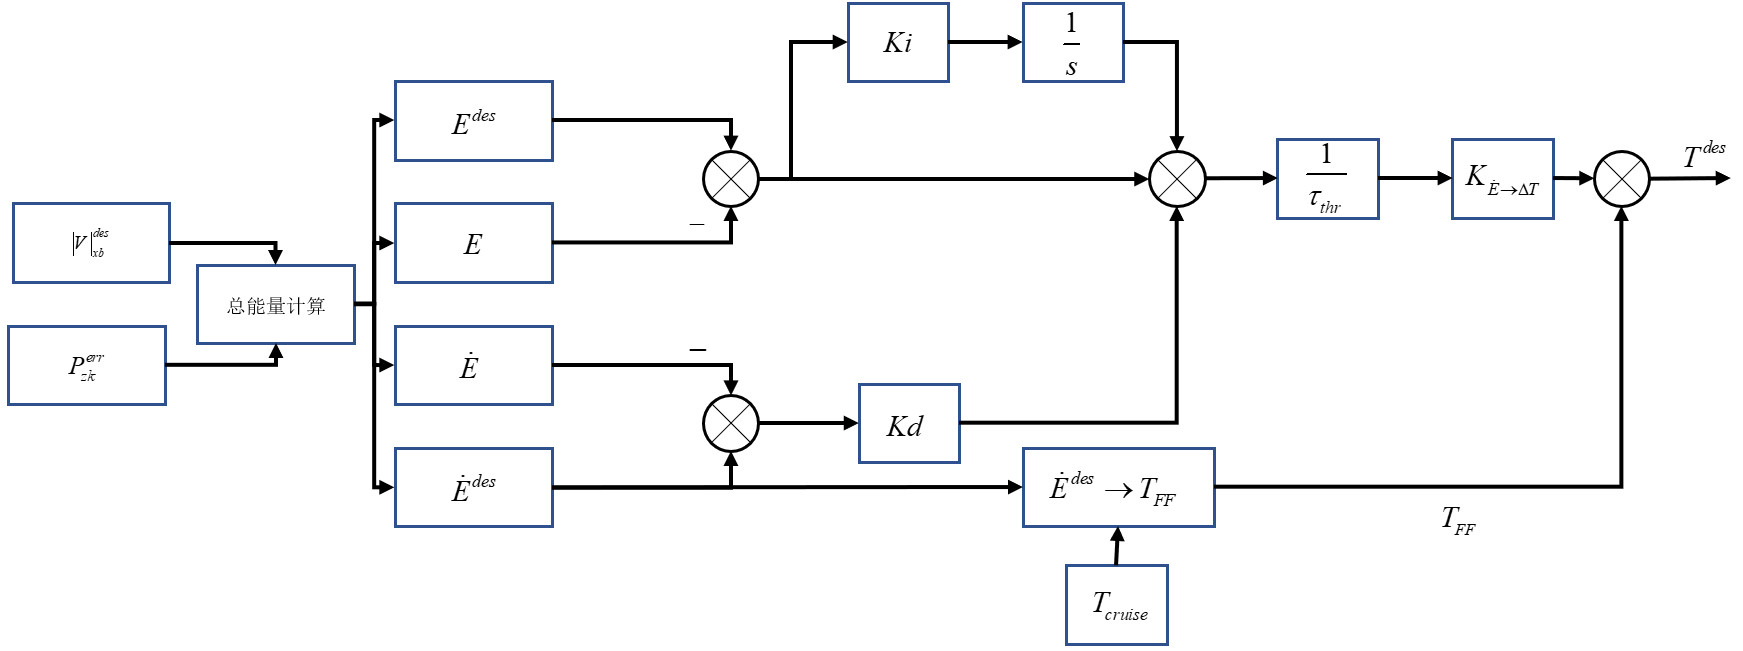
\includegraphics[width=0.9\textwidth]{figures/c3/TECS_throttle.jpg}
    \caption{总能量环}\label{fig:total_energy}
\end{figure}
\begin{figure}[H]
    \centering
    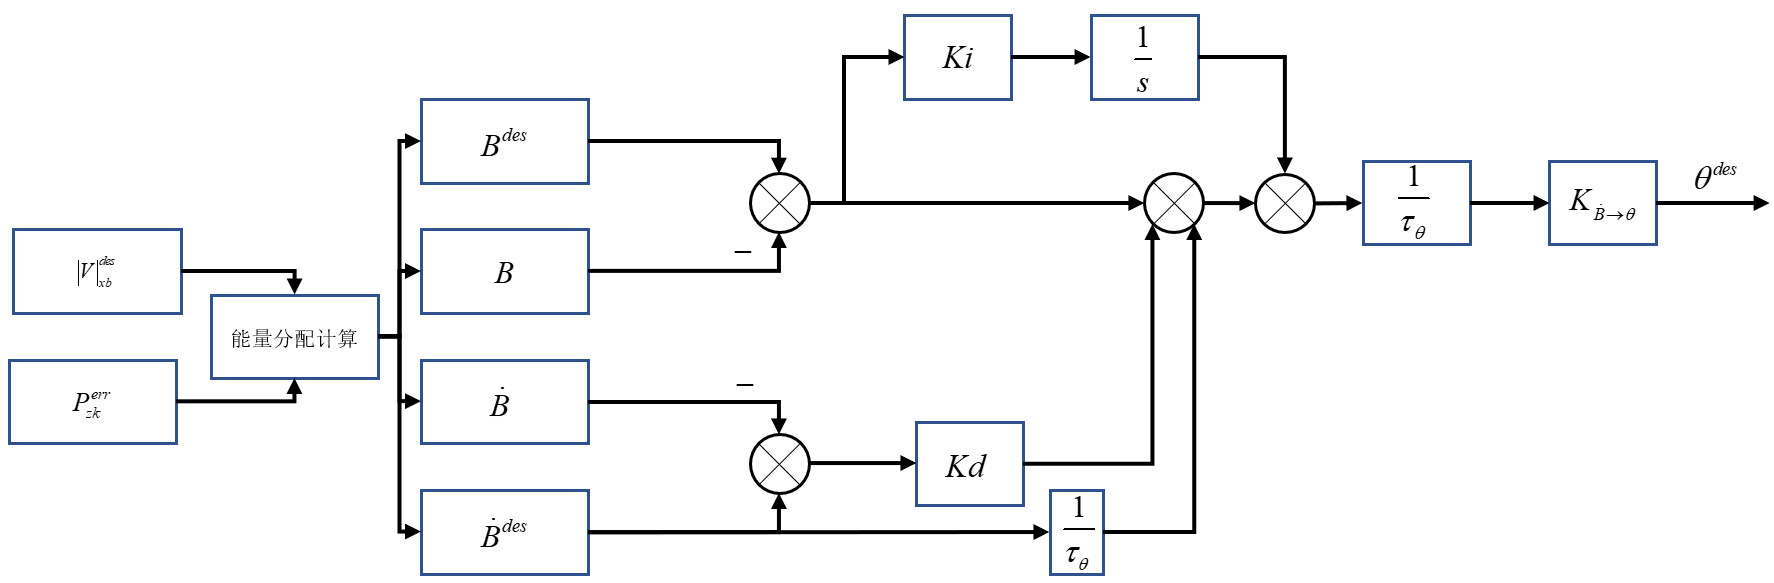
\includegraphics[width=0.9\textwidth]{figures/c3/TECS_pitch.jpg}
    \caption{能量分配环}\label{fig:balance_energy}
\end{figure}
图\ref{fig:total_energy}中,$K_i,K_d,T_{FF},\tau_{thr},K_{\dot{E}\rightarrow\Delta T}$分别为积分项,微分项比例系数,油门前馈项,油门时间常数以及比例向项系数。
图\ref{fig:balance_energy}中,$K_i,K_d,\tau_{\theta},K_{\dot{B}\rightarrow\Delta \theta}$分别为积分项,微分项比例系数,俯仰角时间常数以及比例向项系数。
\subsection{L1控制器实现逻辑}
\section{姿态内环实现原理}
